\section{Approximation Algorithms} \label{s:lpr}

Before a line of classic work of using linear programming (LP) relaxations for designing approximation algorithms of precedence constrained scheduling problems, no constant-factor approximation algorithms were known. In ~\cite{schulz1996scheduling} a 2-approximation algorithms for $1|prec|\sum_j w_jC_j$ is obtained and a 5.3281-approximation algorithms for $P|prec|\sum w_jC_j$ is shown in~\cite{chakrabarti1996improved}. We choose to review the key steps and insights of ~\cite{queyranne2006approximation} in details to show a 4-approximation algorithm for $P|prec|\sum w_jC_j$, since it represents and summarizes this family of algorithms and yields a simple but general framework for the variants of precedence constraints scheduling problems.

The main rounding idea after the LP relaxation is to utilize the solution from LP to construct a priority list of the jobs. Then we can simulate  the time passing forward (to each critical events, e.g., job finished) and schedule the next job in the list, while preserving the capacity constraints and precedence constraints. The construction of such list directly influence the quality of the scheduling. We illustrate in \S\ref{s:lst} and \S\ref{s:lpc}, that a greedy work-conserving job list and the job list from completion time in LP relaxation can lead to very poor result, and actually the midpoint of jobs from LP relaxation leads to the 4-approximation algorithm in \S\ref{s:lpm}.

Unfortunately, the direct LP relaxation of the ILP in \S\ref{s:ilp} is not straightforward to use. If we relax the integer constraint, which captures the job completion time stamp, it breaks the unity of the jobs and thus becomes hard to define the ``mass'' of the jobs for ordering. In order for the LP relaxation to yield a naturally feasible solution, we instead need to use directly the job completion time $C_j$ as the decision variable in \S\ref{s:lprd}, which represents a simplistic way of expressing resource capacity constraints. 

\subsection{List scheduling} \label{s:lst}
LP relaxation for other classic scheduling problem are commonly used with list-scheduling algorithms, which is first introduced in ~\cite{graham1966bounds}. From the solution of the LP relaxation, jobs are sorted based on some rank (e.g., completion time in the solution). Then in the actual scheduling, to satisfy the capacity constraint, whenever a machine becomes available, the next job in the sorted list will be scheduled. To satisfy the precedence constraint\footnote{The job list should not introduce head-of-line blocking, meaning the current head of the job can not be preceded by some job appearing lateral in the list. The feasibility of LP-relaxation solution will prevent this from happening, which will be shown in \S\ref{s:lprd}.}, the next job can only start executing if its predecessors are all finished executing. 

In the presence of precedence constraints, a natural way of assigning job rank is to greedily select the next job if all of its predecessors are already selected. This actually yields a $(2-1/m)$ approximation for the objective of make span ($P|prec|C_{max}$). However, in our weighed completion metric, this can lead to a poor result in the scale of machines counts. 

An example in~\cite{queyranne2006approximation} illustrates this observation: consider $m\geq 3$ machines and three types of jobs, unit-time job $a$, unit-time weight-$1$ jobs $b_1, b_2, ..., b_m$ and m-unit time weight-0 jobs $c_1, c_2, ..., c_{m-1}$. The only precedence constraint is that job $a$ precedes every job in type $b$. The optimal scheduler is to schedule job $a$ first but leave the rest $m-1$ machine idle, so as to schedule type $b$ jobs once $a$ is finished, which leads to its objective value $2m$. The greedy algorithm that keeps resource busy would schedule the jobs of type $c$ in the rest of the machines in the beginning, forcing jobs $b$ being scheduled one after another on the same machine as the job $a$, which results in an objective value $(m+1)(m+2)/2 -1$. Such a greedy list scheduling algorithm is worse than the optimal in the scale of machines $m$ asymptotically.

As the example showed, in some cases we need to deliberately leave an idle time to prevent large-weight jobs, which may become soon in short future, from being blocked by other less important jobs. On the other hand, too much idle time is unnecessary as well. In this sense, LP-relaxation serves as a ``filter" to construct an appropriate job list to balance this tension. 

\subsection{LP-relaxation} \label{s:lprd}
In order to perform LP-relaxation, we now step into another way of expressing the same optimization problem in \S\ref{s:ilp}. The decision variable $C_j$ is kept as in \eqref{eq:ptime} and \eqref{eq:prec}, to capture job duration and the precedence constraints. For machine capacity constraint, we instead write
\begin{align}
\sum_{j\in F} p_j C_j \geq \frac{1}{2m}\left(\sum_{j\in F} p_j \right)^2 + \frac{1}{2}\sum_{j\in F}p_j^2 \:\:\:\: \forall F \subseteq N. \label{eq:mac}
\end{align}
This inequality expresses a convex hull of feasible completion time vectors that captures the constraint, in which each machine can process at most one job at a time. It can be understood in the following derivation. Consider a single machine $i$ and a set of jobs being scheduled in that machine as $F_i$. Without loss of generality, assume the jobs are scheduled are indexed $\{1,2,...,j\} \in F_i$. Since this single machine can only schedule a single job at a time and the job execution is non-preemptive, we have $C_j \geq \sum_{k=1}^j p_k$. Then summing over all jobs in the set, 
\begin{align}
\sum_{j\in F_i} p_j C_j \geq \sum_{j\in F_i} p_j \sum_{k=1}^j p_k = \frac{1}{2} \left[ \left(\sum_{j\in F_i} p_j\right)^2 + \sum_{j\in F_i}p_j^2\right]. \label{eq:ch}
\end{align}

Summing over all machines, the second term in the last expression becomes directly $\sum_{i=1}^m \sum_{j\in F_i}p_j^2 = \sum_{j\in F}p_j^2$, and the first term indicates $\sum_{i=1}^m\left(\sum_{j\in F_i} p_j\right)^2 \geq \frac{1}{m}\left(\sum_{j\in F} p_j\right)^2$, due to Cauchy-Schwarz inequality. 

Notice that the relaxation occurs to this linear program when we enforce $F$ to be \emph{any} subset in $N$. Altough there is an exponential number of constraints in \eqref{eq:mac}, \cite{queyranne2006approximation} points out that the separation problem for these inequalities can be solved in polynomial time, thus this LP relaxation can be solved in polynomial time, using ellipsoid method. Because of the scope and the length limit, we refer the proof to \cite{schulz1996scheduling}.

Notice that the solution of the LP relaxation is a feasible solution for the scheduling problem satisfying the precedence and machine capacity constraints. In order for the list-scheduling in \S\ref{s:lst} to present a feasible solution, the ordering of the jobs in the list needs to avoid head-of-line blocking, i.e., the scheduling of the next job in the list is constrained by a job presented lateral in the list. In fact, ordering the job in the list based on any ``location'' of the job $C_j - \alpha p_j$ for any $\alpha \in [0,1]$ would avoid head-of-line blocking. This is because the blocking requires a job $i$ precedes job $j$ and $i$'s finish time is ahead of $j$'s starting time. Thus picking a location anywhere in the interval of the job preserves the precedence ordering in the list.

\subsection{Ranking on the completion time} \label{s:lpc}
A straightforward way of utilizing LP-relaxation solution is to order the jobs based on their completion time. However, it turns out this can lead to very poor schedules in a meticulously designed example. We consider $m \geq 2$ machines and $m$ sets of jobs $J_h, h\in\{1,2,..,m\}$. Each set $J_h$ contains a long job of processing time $1 + (h-1)(m+1)\epsilon$, $m$ small jobs with processing time $\epsilon$ each. Additionally, there is a final job preceded by all the jobs. The weights of the jobs are all $0$ except for the last job. The precedence constraints are imposed independently on each job set, from the long job to all small jobs. The existence of this final job is to transform the problem from minimizing $\sum_jw_jC_j$ to minimizing makespan $C_{max}$. The construction is illustrated in figure~\ref{fig:lpc}.

\begin{figure}[h]
\centering
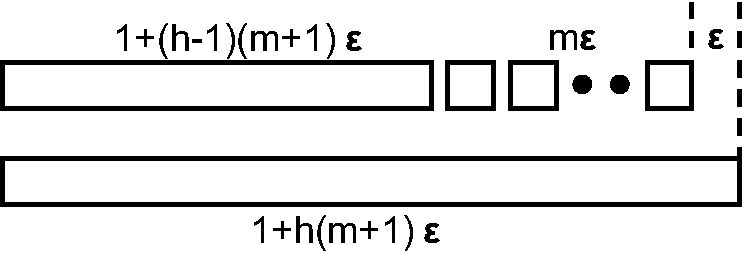
\includegraphics[width=0.5\textwidth]{figs/lpc.pdf}
\caption{List scheduling using the completion time from LP relaxation can lead to poor result in the scale of machines. This example constructs set of small jobs squeezes in front of big jobs as their completion times are earlier.}
\label{fig:lpc}
\end{figure}

The optimal schedule would schedule each long job at the beginning on each machine, then finish all the small jobs in its group immediately one after another. The makespan in this case is effectively the completion time of the last small job of the job set with longest job, which is $(1 + m(m+1)\epsilon) + m\epsilon = 1 +(m^2+2m)\epsilon$. 

Notice that in the optimal solution, each small job in the job set $J_{h-1}$ has completion time earlier than the long job in the next job set $J_h$, as shown in figure~\ref{fig:lpc}. Also, the LP formulation in \S\ref{s:lprd} will find this solution because at the first time step, reaching the solution to the extreme point is to schedule all long jobs (no other jobs can be scheduled because of the precedence constraint), which yields the smallest objective directly. Then putting the priority list with the completion time of the jobs means we put the small jobs of set $J_h$ ahead of the long jobs in the next set $J_{h+1}$. Now scheduling from the list blocks the long job in $J_{h+1}$ being scheduled until all small jobs in $J_h$ finish executing, for every $h$. Therefore, the starting of the long job in $J_h$ is delayed by at least $h$, as it needs to at least wait for all long job in $J_{1, 2,.., h-1}$ to finish. This results in a makespan at least $\sum_h 1 + (h-1)(m+1)\epsilon = m + o(\epsilon)$, which is effectively $m$ times worse than the optimal for sufficiently small $\epsilon$.

\subsection{Ranking on the midpoint} \label{s:lpm}
Instead of sorting the job based on completion time solution in LP relaxation, we use the midpoint from the result. The midpoint is defined as $M_j = C_j - p_j/2$. This results in a 4-approximation approximation algorithm for $P|prec|\sum w_jC_j$ as following: Let $C^{LP}$ denotes any feasible solution to the LP relaxation in \S\ref{s:lprd} and $M^{LP}$ denotes the corresponding vector of LP midpoints, let $S_j$ be the vector of start times of the feasible solution constructed by list scheduling using LP midpoints, then

\begin{align}
S_j \leq 4 M^{LP}_j \:\:\:\: \forall j \in N
\end{align}

The proof for this statement can be conducted by separately considering the ``busy hours" and ``free time'' of the machines. Specifically, we denote $\mu$ as the total time before $S_j$ that \emph{all} machines are occupied by some other jobs. This separate the time span before $S_j$ into two kinds of period, busy and idle. We then separately show that the aggregation of all busy period and idle period are \emph{both} bounded by $2M^{LP}_j$. Namely, we are to show $\mu \leq 2 M^{LP}_j$ and  $S_j - \mu \leq 2 M^{LP}_j$.

The busy period is relatively straightforward. Notice that $\mu$ is upper bounded by $\sum_{i=1}^{j-1} p_i /m$, because the longest consecutive busy hour can be bounded by liquidizing the processing time of all jobs prior to $j$ and assigning them uniformly to all machines. Notice that in \eqref{eq:ch}, if we rearrange the last term in the RHS to the LHS and observe the definition of midpoint $C_j-pj/2 = M_j$, we will have 
\begin{align}
\left(\sum_{i=1}^{j-1}p_i\right)M^{LP}_j \geq \sum_{i=1}^{j-1} p_i M^{LP}_i \geq \frac{1}{2m}\left(\sum_{i=1}^{j-1}p_i\right)^2,
\end{align}
which leads to $\mu \leq \sum_{i=1}^{j-1} p_i /m \leq 2 M^{LP}_j$ as desired. 

\begin{figure}[h]
	\centering
	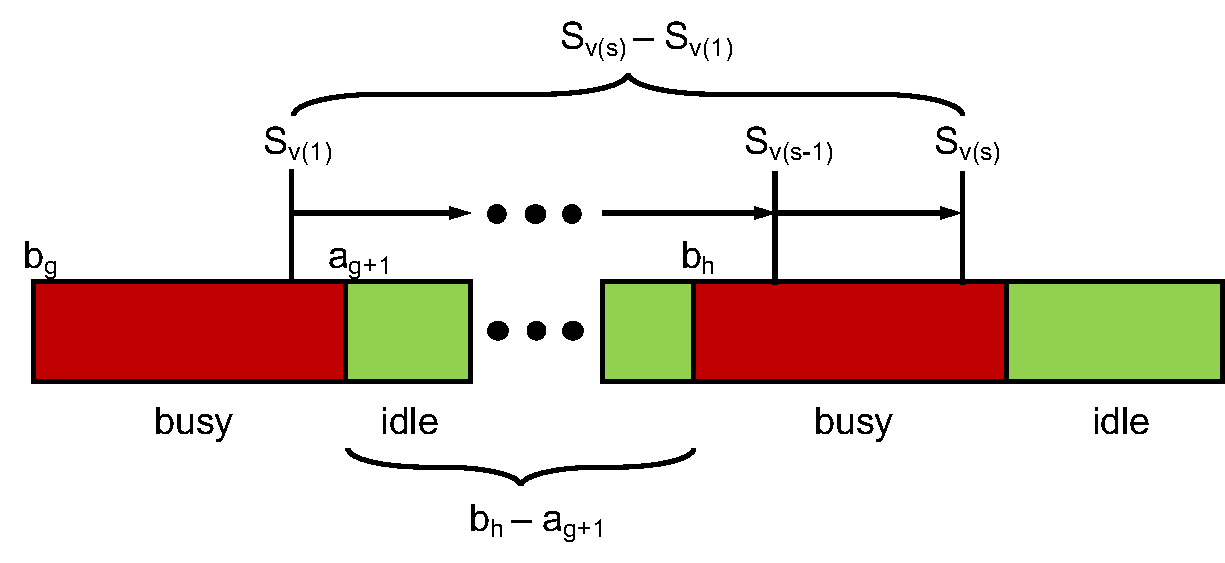
\includegraphics[width=0.6\textwidth]{figs/4-approx-1.pdf}
	\caption{Bound the machine idle period using a set of consecutively scheduled jobs.}
	\label{fig:4-approx}
\end{figure}

On the other hand for the idle period, we aim to show $S_j - \mu \leq 2 M^{LP}_j$, where the LHS is the aggregation of the time period in which at least one machine is idle. The way of reaching this bound is to group the job set that is consecutively running one after another, which in order words saturates the precedence constraints in \eqref{eq:prec}. Specifically, we denote the idle periods as $[a_h, b_h]$. Then starting from $S_j$, we walk backwards in time, and encounter the first busy period with $b_h$ on its left boundary. We denote $v(1), v(2) .., v(s)$ as the \emph{longest} job span with $v(s)$ has its starting time $S_{v(s)}$ in this encountered busy interval and $S_{v(1)}$ falls \emph{out} of the busy interval $S_{v(1)} < b_h$. The span of the consecutive jobs is illustrated in figure~\ref{fig:4-approx}. 

First notice that such $v(1)$ exists, because we know a job starts executing at the boundary $b_h$, and we can at least uses that job as $v(s)$. This job must br preceded on some previous job $v(s-1)$ otherwise it could have been scheduled earlier than $b_h$, since the interval to the left is idle. Secondly, $S_{v(1)}$ has to reside in a busy period $[b_g, a_{g+1})$, otherwise some machine is idle immediately before the execution of $S_{v(1)}$ and it could have been scheduled earlier. Therefore, as shown in figure~\ref{fig:4-approx}, the span of these consecutive jobs captures some idle periods in the middle. This gives us 
\begin{align}
b_h - a_{g+1} \leq S_{v(s)} - S_{v(1)} = \sum_{i=1}^{s-1}(S_{v(i+1)} - S_{v(1)}) = \sum_{i=1}^{s-1} p_{v(i)}. \label{eq:jobset}
\end{align}

Now we can keep on constructing such consecutive job set spanning the next idle period backward in time, starting inside the busy period of $[b_g, a_{g+1})$ in figure~\ref{fig:4-approx}. The reason is that we can find another starting job time inside the busy period, which has its predecessor starts before $b_g$, because we can again at least use the job starts at $b_g$ as a new $v(s')$. From the same argument above we know the consecutive job list begins at another busy period. This way, we can add up all the consecutive time spans to cover all the idle periods. 

Meanwhile, the precedence constraints in \eqref{eq:prec} implies
\begin{align}
M^{LP}_{v(i+1)} \geq M^{LP}_{v(i)} + \frac{1}{2}p_{v(i)} + \frac{1}{2}p_{v(i+1)}. \label{eq:prec2}
\end{align}

Now \eqref{eq:jobset} and \eqref{eq:prec2} can be combined to reach,
\begin{align}
M^{LP}_{v(s)} - M^{LP}_{v(1)} = \sum_{i=1}^{s-1} \left(M^{LP}_{v(i+1)} - M^{LP}_{v(i)}\right) \geq \frac{1}{2}\sum_{i=1}^{s-1} p_{v(i)} \geq \frac{1}{2} (b_h-a_{g+1}),
\end{align}
which now allows us to aggregate all idle periods and to telescope the consecutive job sets to bound the aggregation of $[a_1, b2), [a2, b3), .., [a_{h-1}, b_h)$ by $2M_j^{LP}$. 

Now combining both the busy and idle period, we reach $\mu + (S_j - \mu) \leq 2M_j^{LP} + 2M_j^{LP} = 4M_j^{LP}$, which yields the 4-approximation algorithm.
